\chapter{Dettagli implementativi}

In questo capitolo verranno descritti i pattern principali usati durante la progettazione e lo sviluppo del softaware e le motivazioni che hanno portato a tali scelte.

\section{Custom container controller}
Il \emph{Container View Controller} è un pattern di progettazione iOS che permette di scomporre le applicazioni in parti più piccole e semplici, ognuna delle quali è dedicata ad assolvere un determinato compito. I container controller sono usati quindi come intermediari tra queste diverse parti (\emph{child controller}) allo scopo di fornire un'interfaccia che sia coerente con il contesto in cui i controller figli operano.

\begin{figure}[!htbp]
\centering
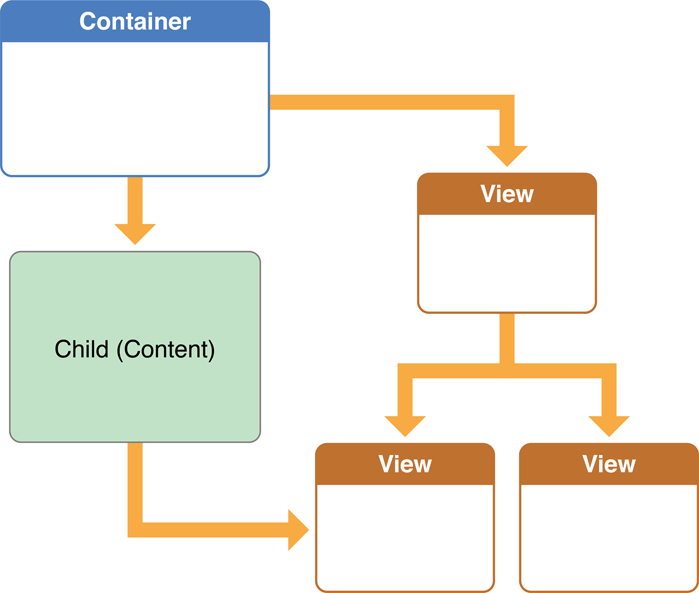
\includegraphics[scale=0.30]{architettura/container.png}
\caption{Schema del \emph{contaier controller design}}
\label{fig:selettore}
\end{figure}

L'utilizzo di tale pattern ha permesso durante la progettazione dell'applicazione di ottenere controller più puliti sotto il punto di vista implementativo ed efficienti sotto il punto di vista delle prestazioni.

\subsection{MiaSituazioneContainerController}
\label{parag:miasituaz}
Uno dei requisiti funzionali principali dell'applicazione prevede la visualizzazione dei conti e carte di un utente e l'eventuale visualizzazionei dei movimenti ad essi relativi.

La parte dell'architettura realizzata per realizzare tali funzionalità è composta dalla seguente gerarchia di container e child controller:

\begin{itemize}
 \item MiaSituazioneContainerController (figura \ref{fig:miasituazione}): è il container controller che ha il compito di creare l'interfaccia di base e di creare un array di child controller:
 \begin{itemize}
  \item ContiContainerController: è il container che gestisce la creazione e la comunicazione tra i controller adibiti alla visualizzazione dei prodotti bancari come vista a bolle o vista a tabella (nello specifico \emph{BubbleViewController} e \emph{ContiTableViewController})
  \item MovimentiContainerController: è il container che gestisce la creazione e la comunicazione tra i controller adibiti alla visualizzazione dei movimenti di un determinato conto (nello specifico \emph{TimelineViewController} e \emph{MovimentiTableViewController})
  \item ContiFilterTableViewController: il controller che si occupa della visualizzazione e della logica di filtraggio dei conti che l'utente può visualizzare a schermo
 \end{itemize}
\end{itemize}
\begin{figure}[!htbp]
\centering
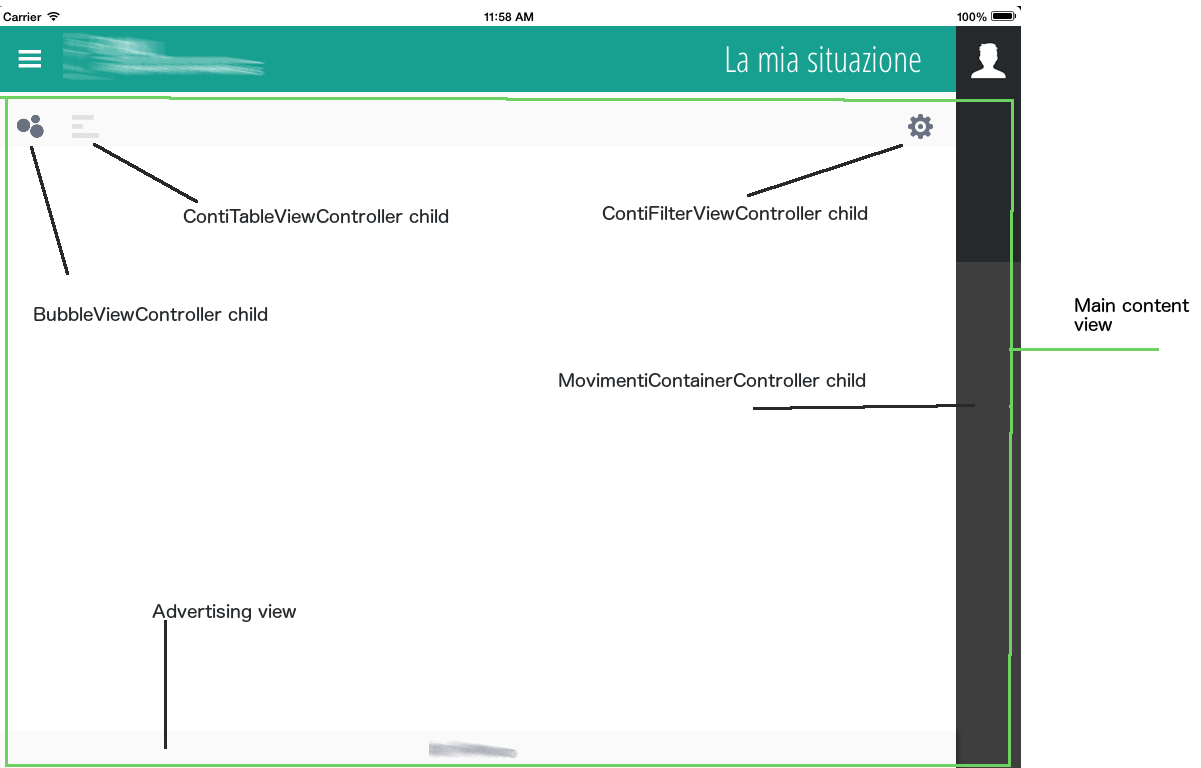
\includegraphics[scale=0.35]{dettagli/miasituazione.png}
\caption{Dettaglio componenti gestiti da MiaSituazioneContainerController}
\label{fig:miasituazione}
\end{figure}
\begin{figure}[!htbp]
\centering
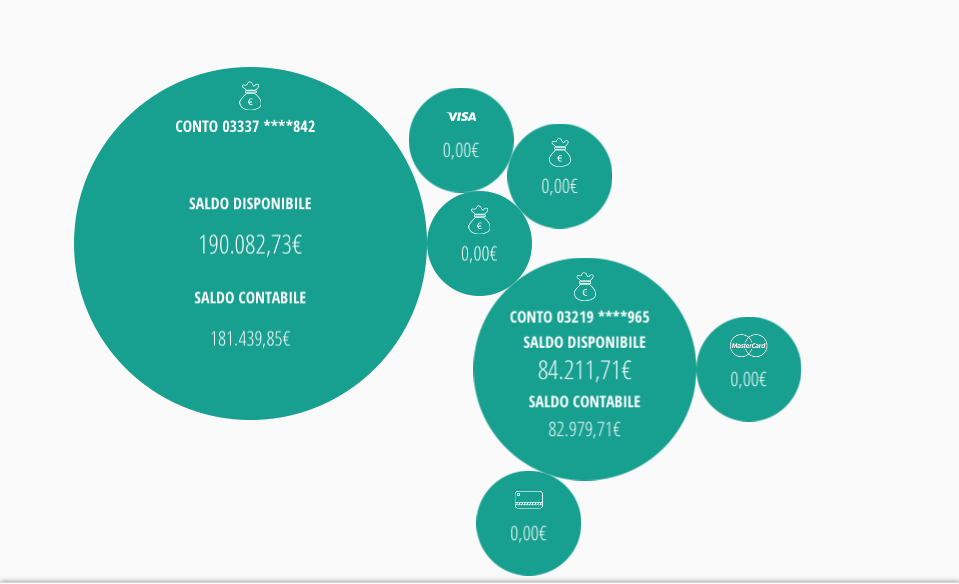
\includegraphics[scale=0.35]{dettagli/bubble.png}
\caption{BubbleViewController}
% \label{fig:miasituazione}
\end{figure}
\begin{figure}[!htbp]
\centering
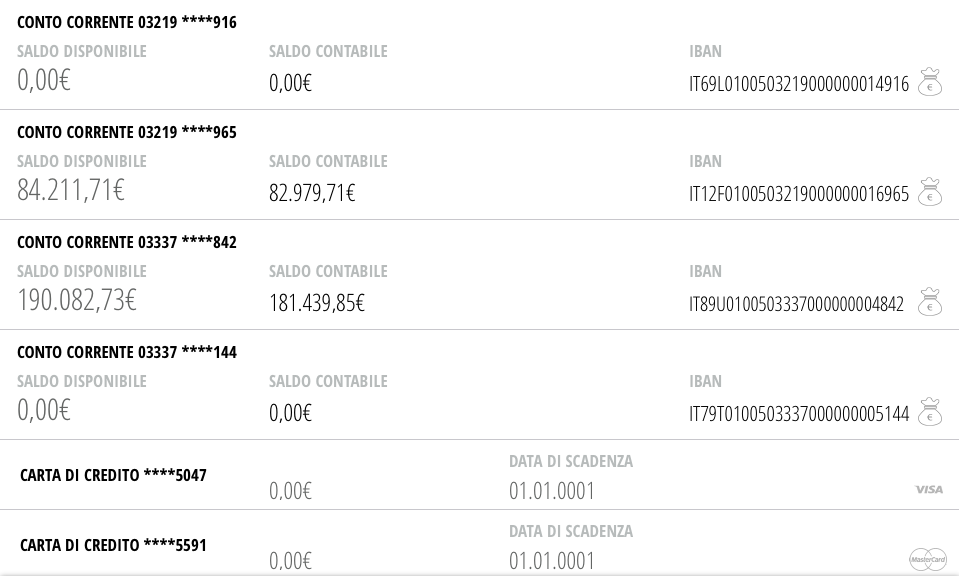
\includegraphics[scale=0.35]{dettagli/contiList.png}
\caption{ContiTableViewController}
% \label{fig:miasituazione}
\end{figure}
Quando \emph{MiaSituazioneContainerController} viene istanziato è eseguita una chiamata ai servizi per ottenere la lista dei conti dell'utente, tale lista verrà quindi utilizzata come model comune a tutta la gerarchia dei controller descritti sopra. È compito quindi del MiaSituazioneContainerController gestire gli eventi dell'interfaccia principale e passare il model a uno dei controller figli quando l'utente sceglierà una delle modalità di visualizzazione descritte precedentemente. 

\subsection{MovimentiContainerController}

Come brevemente descritto nel paragrafo \ref{parag:miasituaz} tale container ha il compito di gestire i child controller adibiti alla visualizzazione dei movimenti di un conto. 
Nello specifico tale container si occupa della gestione ad alto livello delle funzioni e degli eventi relativi ai componenti dell'interfaccia da esso gestiti (figura \ref{fig:movimenticontainer}). A titolo illustrativo esso gestisce gli eventi scatenati dal selettore dei conti e dal filtro calendario; in particolare ad ogni cambio di conto o di data del filtro il MovimentiContainerController effettua una chiamata ai servizi per ottenere una lista di movimenti che verrà utilizzata come model comune a tutti i figli di tale container.

\begin{figure}[!htbp]
\centering
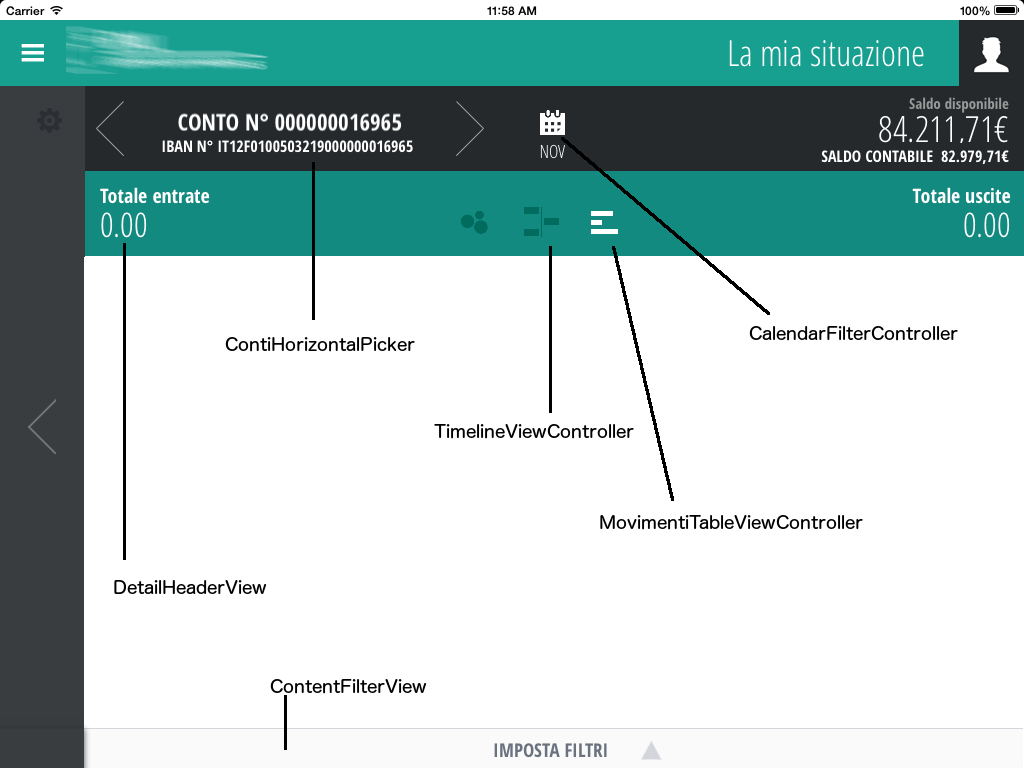
\includegraphics[scale=0.35]{dettagli/movimenticontainer.png}
\caption{Dettaglio dei componenti gestiti dal controller MovimentiContainerController}
\label{fig:movimenticontainer}
\end{figure}

\subsection{Comunicazione tra container e child controller}
I container controller sono gli unici componenti consapevoli dell'esistenza di altri controller nella gerarchia, in particolare dei child controller da loro direttamente creati.
I child controller sono realizzati quindi come componenti indipendenti che non hanno percezione del controller padre o dei loro fratelli. 

La comunicazione tra i container e i suoi figli è stata realizzata in modo tale da garantire sempre un'elevata modularità dell'architettura mediante l'utilizzo dei pattern messi a disposizione dall'SDK iOS:

\begin{itemize}
 \item message passing: realizza la comunicazione in avanti tra un container e un child controller mediante opportune interfacce messe a disposizione dai child contoller
 \item pattern delegate: realizza la comunicazione all'indietro da un child ad un container controller mediante la dichiarazione di opportuni protocolli (\emph{protocol} nella tecnlogia iOS) da parte dei child controller. I container controllor vengono quindi dichiarati conformi a tali protocolli e posti come \emph{delegate} ( oggetti che operano come aiutanti adibiti all'esecuzione di compiti particolari)
\end{itemize}

L'adozione di tali pattern durante la progettazione ha permesso di ottenere un'architettura modulare composta da componenti specializzati facilmente estendibili e riusabili.

\newpage
\begin{figure}[!htbp]
\centering
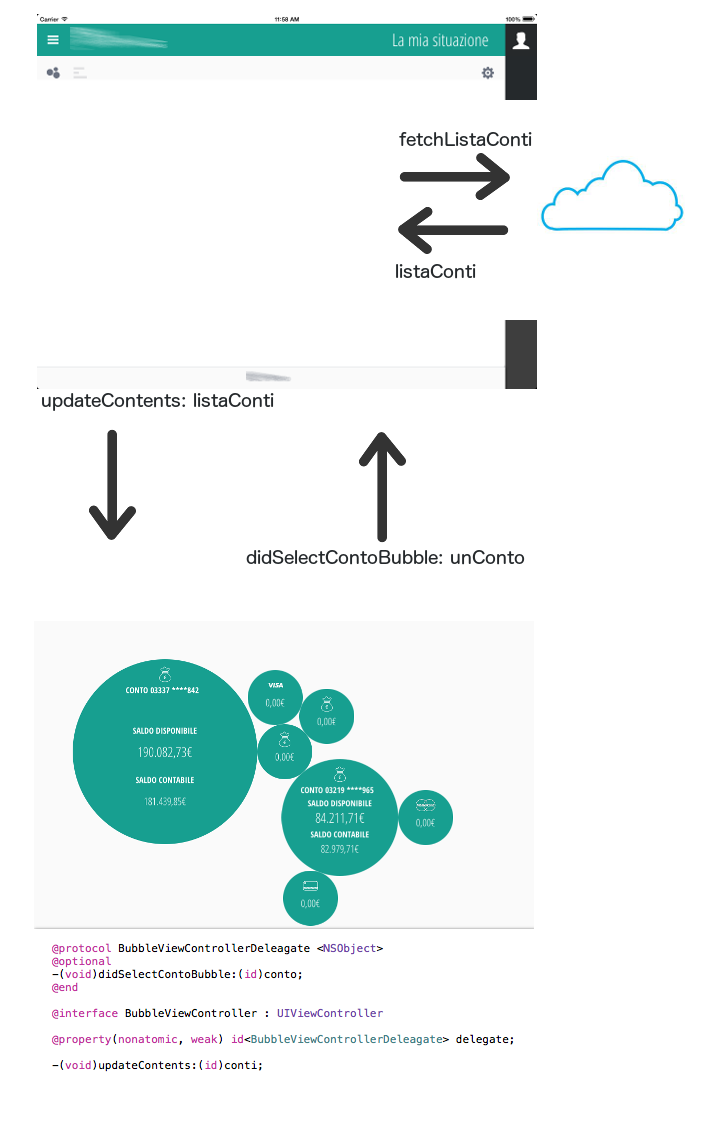
\includegraphics[scale=0.6]{dettagli/communication.png}
\caption{Esempio di comunicazione da un container padre a un child controller}
\label{fig:movimenticontainer}
\end{figure}
